\documentclass[10pt]{article}
\usepackage[margin=0.85in]{geometry}
\usepackage[T1]{fontenc}
\usepackage{lmodern}
\usepackage{microtype}
\usepackage{amsmath,amssymb,amsthm}
\usepackage{booktabs,graphicx}
\usepackage[numbers,sort&compress]{natbib}
\usepackage[colorlinks=true,linkcolor=blue,citecolor=blue,urlcolor=blue]{hyperref}
\newtheorem{proposition}{Proposition}
\newcommand{\E}{\mathbb{E}}
\newcommand{\one}{\mathbf{1}}
\title{When Local Credit Assignment Breaks:\\Exact Diagnostics of Additive and Pairwise Reward Projection}
\author{Varun Kasamneni}
\date{October 1, 2026\\\small Research manuscript draft; not submitted or peer reviewed}
\begin{document}
\maketitle
\begin{abstract}
Average reward reconstruction error is an incomplete measure of the decision quality of a factored cooperative model. We provide a small, fully reproducible diagnostic of this established issue, rather than a new multi-agent reinforcement learning algorithm. In a binary one-step game with a rare joint synergy, the exact uniform least-squares additive projection has mean squared error $2^{-n}-(n+1)4^{-n}$ but coordination regret $1-3n2^{-n}$. Adding any set of pairwise factors reduces reconstruction error without changing the wrong maximizing action. Exhaustive evaluation at up to 16 agents confirms the formulas; 800 independent sampled fits illustrate that observing the synergistic action need not repair the population projection objective. A privileged twofold weight on the known optimal action reverses the policy while increasing uniform reconstruction error. At 16 agents, additive MSE is $1.52548\times10^{-5}$ and regret is $0.999268$. However, MSE divided by reward variance is $0.999939$, exposing the apparently small absolute error as a sparse-reward averaging effect. The package supplies proofs, controlled ablations, an established matrix-game check, raw results, and tests. It does not reproduce LOMAQ or establish a new failure of neural value-decomposition algorithms.
\end{abstract}

\section{Introduction}
Cooperative agents often learn from a joint reward while selecting actions through restricted local utilities. A common diagnostic asks whether the aggregate prediction reconstructs that reward. The practical question is whether the prediction preserves the decisions that matter. These objectives differ: averaging errors over a large action space can conceal a severe error at one valuable coordinated action.

This observation is not new. Weighted QMIX explicitly analyzes how unweighted projection can select an incorrect action even with access to the true joint value function~\cite{rashid2020weighted}. Our contribution is a compact, executable diagnostic that makes the scaling, topology, metric normalization, and sampling effects inspectable without neural optimization. We give a closed-form family with bounded reward range, evaluate the complete action population, and retain every finite-sample fit. The resulting package can test evaluation procedures before more expensive MARL experiments. We do not claim first discovery of the reconstruction--decision gap, algorithmic superiority, or a complete MARL benchmark.

\section{Related work and scope}
VDN learns an additive decomposition of team values~\cite{sunehag2018vdn}. QMIX uses monotonic mixing so that maximizing individual utilities is consistent with maximizing its represented joint value~\cite{rashid2018qmix}. QTRAN studies a broader transformation-based factorization criterion~\cite{son2019qtran}. These are learning systems; the present additive least-squares estimator only shares a restricted function class with VDN.

Weighted QMIX is the closest conceptual precedent: its projection analysis separates reconstruction from action selection and motivates weighting valuable actions~\cite{rashid2020weighted}. Our oracle-anchor ablation is a linear, analytically solvable illustration of that idea, not an implementation or improvement of Weighted QMIX. Deep Coordination Graphs models pairwise payoffs and uses message passing~\cite{boehmer2020dcg}; our graph projections instead use exact central enumeration to remove inference error.

LOMAQ exploits local rewards together with structural assumptions supporting cooperative maximization, and its reward-decomposition study already illustrates locality misspecification~\cite{zohar2022lomaq}. Our counterexample does not contradict its conditional guarantees: our game intentionally contains an interaction involving every agent. A recent preprint also studies local rewards with dependence graphs~\cite{le2026explicit}; it is related context, not an evaluated baseline. This focused literature review is not an exhaustive novelty survey. No claim is made that the present elementary construction is unprecedented.

\section{Diagnostic and estimators}
There is one state, one simultaneous joint action $a\in\{0,1\}^n$, and a common deterministic reward. Agent identities are fixed; there are no observation or transition dynamics. Define
\begin{equation}
 R_{n,\kappa}(a)=\one\{a=\one^n\}-\kappa 2^{1-n}\sum_{i=1}^n a_i.\label{eq:game}
\end{equation}
The main setting is $\kappa=3/2$ and $n\geq4$. The unique optimal action is $\one^n$, with reward $1-3n2^{-n}>0$; every other nonzero action has negative reward, and $R(\mathbf0)=0$. The reward range is $1-3\cdot2^{-n}<1$ and approaches one. Thus the central result is not produced by uniformly shrinking the reward scale, although the large reward becomes rare under uniform sampling.

Let $x_i=2a_i-1$ and $p=2^{-n}$. For an edge set $G$, the approximation class is
\begin{equation}
 \widehat R_G(a)=b_0+\sum_i b_i x_i+\sum_{(i,j)\in G}b_{ij}x_ix_j.\label{eq:model}
\end{equation}
The additive model has $G=\varnothing$. Other graphs are a chain, ring, star, and complete graph. We minimize the uniform population squared error exactly. Walsh features in (\ref{eq:model}) are orthonormal under this distribution, so each fitted coefficient is its reward inner product. In finite-sample experiments, ordinary least squares uses only sampled feature rows and rewards.

The additive greedy policy is independently executable: agent $i$ chooses $a_i=1$ if $b_i>0$, otherwise zero. Pairwise predictions are maximized by exhaustive centralized search. This is an optimistic inference diagnostic and does not implement decentralized graph coordination. Ties within absolute tolerance $10^{-12}$ select the first binary index; the $\kappa=1$ stratum is explicitly a tie case.

Our primary metrics are
\begin{equation}
 L=\E_{a\sim U}(\widehat R(a)-R(a))^2,\qquad
 \mathcal R=\max_a R(a)-R(\arg\max_a\widehat R(a)).
\end{equation}
We also report $L/\operatorname{Var}_U(R)$, range-normalized RMSE, maximum absolute error, and optimal-action success. The variance-normalized measure is essential: small absolute MSE does not imply that substantial reward variation was explained.

\section{Analytical properties}
\begin{proposition}[Sparse synergy projection]\label{prop:main}
For $\kappa=3/2$ and $n\geq4$, the unique uniform projection onto (\ref{eq:model}) has $b_0=p(1-3n/2)$, $b_i=-p/2$, and $b_{ij}=p$. Its unique maximizing action is $\mathbf0$, for every edge set $G$. Moreover,
\begin{equation}
 L_G=p-(1+n+|G|)p^2,\qquad \mathcal R_G=1-3np.
\end{equation}
Consequently $L_G\to0$ and $\mathcal R_G\to1$ for additive and pairwise graph sequences, including complete graphs.
\end{proposition}
\begin{proof}
The synergy indicator equals $p\prod_i(1+x_i)$ and has coefficient $p$ for every Walsh subset. The cost is $(3np/2)+(3p/2)\sum_i x_i$. Projection keeps the constant, singleton, and selected pair terms, yielding the stated coefficients. All omitted terms have coefficient $p$, so orthogonality gives the error as the number of omitted terms times $p^2$. At $x_i=-1$ every negative singleton term is maximized, and every positive pair term is also maximized. The strictly negative singleton coefficients make this joint maximizer unique. Its true reward is zero, proving the regret formula. Finally, $|G|\leq n(n-1)/2$, so the error vanishes exponentially.
\end{proof}

For general $\kappa$, the singleton coefficient is $(1-\kappa)p$. The population MSE is independent of $\kappa$ because the entire changing cost lies inside every approximation class. For $\kappa<1$ all singleton and pair coefficients favor $\one^n$, whereas $\kappa>1$ favors $\mathbf0$. This isolates a policy transition invisible to unnormalized reconstruction MSE.

\paragraph{Why normalization matters.}
At $\kappa=3/2$, the additive variance-normalized error is
\begin{equation}
 \frac{L}{\operatorname{Var}(R)}=
 \frac{2^n-n-1}{2^n-n-1+n/4}\longrightarrow1.
\end{equation}
This is not a case of strong explained-variance accuracy accompanied by poor decisions. It is a counterexample to using absolute distribution-average error as a decision certificate. In contrast, if $\|R-\widehat R\|_\infty\leq\epsilon$, the usual two-error argument gives $\mathcal R\leq2\epsilon$. From uniform MSE alone one obtains only $\mathcal R\leq2\sqrt{2^nL}$, which is uninformative here.

\paragraph{Privileged weighting ablation.}
Give the known optimal action weight $w\geq1$ and all other population actions weight one when fitting the additive model. If $v=(1,\ldots,1)^\top\in\mathbb R^{n+1}$, the fitted coefficients become
\begin{equation}
 b^{(w)}=b+\delta v,\quad
 \delta=\frac{(w-1)[1-(n+1)p]}{2^n+(w-1)(n+1)}.\label{eq:anchor}
\end{equation}
This follows from a rank-one update to the orthogonal design Gram matrix. When $w=2$ and $n\geq4$, $2^n>3(n+1)$ implies $\delta>p/2$: every unary coefficient becomes positive, giving zero regret. Yet the uniform MSE increases by $(n+1)\delta^2$. This is a demonstration of objective mismatch using privileged knowledge, not a practical solution for finding the rare action.

\section{Experimental protocol}
The local protocol and configuration were written before execution and retained with SHA-256 hashes; they were not publicly preregistered. Theory determined the task design and parameter choices. We first ran 33 tests and a separate smoke pilot. The fixed main run comprised 96 exact evaluations, 800 sampled fits, and three controls; no runs failed or were excluded.

The scaling experiment used $n\in\{4,6,8,10,12,14,16\}$, five graph classes, and oracle-anchor weights $2,16,256$. The strength ablation fixed $n=8$ and used $\kappa\in\{0,0.5,0.9,1,1.1,1.5,2,3\}$. The finite-coverage experiment used $n\in\{8,12\}$, sample sizes $m\in\{64,256,1024,4096\}$, and 100 independent uniform-with-replacement datasets per cell. No hyperparameters were tuned. Full-population evaluation intentionally includes training actions; this is a projection/coverage diagnostic, not a claim of held-out task generalization. The fitting function receives only training features and targets; the separately labeled oracle-anchor variant additionally receives privileged population information.

Datasets, not joint actions within a dataset, are the sampling units. We report Wilson 95\% intervals for proportions and descriptive normal 95\% intervals for mean regret across the 100 datasets. One hundred replicates give a worst-case binomial standard error of 0.05; the study is not powered to certify small improvements. Exact population results require no uncertainty intervals. All sample indices are regenerable from retained seeds and their byte-level hashes; fitted coefficients and per-run metrics are retained.

Implementation uses NumPy 2.5.3 with float64 arrays; figures use Matplotlib 3.11.2. The manifest records Python, OS, architecture, logical CPU count, source hashes, and individual runtimes. The main run completed in approximately 0.27 seconds of measured in-process time on a Darwin arm64 environment with 12 logical CPUs; this excludes dependency installation, plotting, testing, and manuscript work. No accelerator or paid API was used. This timing is a reproducibility record, not a speed comparison. A separate pilot took approximately 1.55 seconds, illustrating that timings of these small runs are noisy.

\section{Results}
\subsection{Scaling and topology}
Figure~\ref{fig:scaling} and Table~\ref{tab:scaling} show vanishing absolute error with persistent decision failure. At $n=16$, the additive model has MSE $0.0000152548$ and regret $0.999268$. Complete pairwise factors reduce MSE to $0.0000152269$ without reducing regret. The maximum reconstruction error remains large: Proposition~\ref{prop:main} reflects concentration of the missed interaction at the rare joint action, not uniform predictive accuracy. Normalized MSE approaches one, correctly indicating weak reconstruction of reward variation.

\begin{figure}[t]
\centering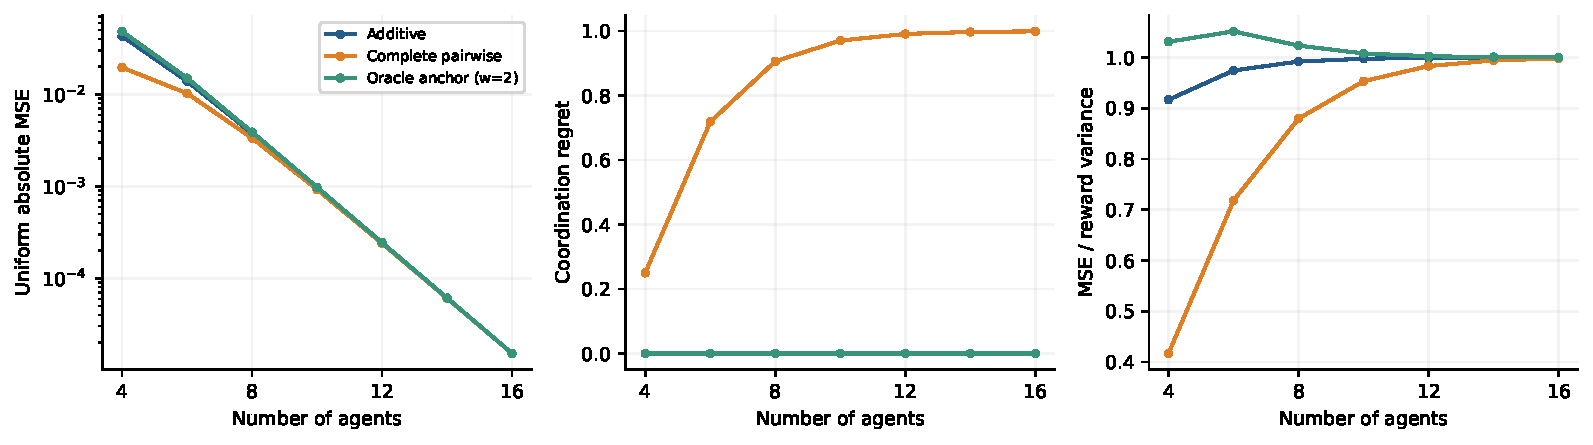
\includegraphics[width=\linewidth]{../figures/scaling.pdf}
\caption{Exact population diagnostics at $\kappa=1.5$. Additive and complete-pairwise regret curves coincide. The oracle-anchor estimator knows which action is optimal and doubles its weight. It achieves zero regret despite slightly higher uniform MSE; its normalized MSE can exceed one. There are no sampling error bars in this exhaustive experiment.}\label{fig:scaling}
\end{figure}

\begin{table}[t]\centering\small
\begin{tabular}{rllrrr}
\toprule
Agents & Model & Weight & MSE & MSE/Var & Regret \\
\midrule
4 & Additive & 1 & 0.0429688 & 0.9167 & 0.250000 \\
4 & Pairwise & 1 & 0.0195312 & 0.4167 & 0.250000 \\
4 & Oracle anchor & 2 & 0.0483277 & 1.0310 & 0.000000 \\
8 & Additive & 1 & 0.00376892 & 0.9920 & 0.906250 \\
8 & Pairwise & 1 & 0.00334167 & 0.8795 & 0.906250 \\
8 & Oracle anchor & 2 & 0.00388823 & 1.0234 & 0.000000 \\
12 & Additive & 1 & 0.000243366 & 0.9993 & 0.991211 \\
12 & Pairwise & 1 & 0.000239432 & 0.9831 & 0.991211 \\
12 & Oracle anchor & 2 & 0.000244131 & 1.0024 & 0.000000 \\
16 & Additive & 1 & 1.52548e-05 & 0.9999 & 0.999268 \\
16 & Pairwise & 1 & 1.52269e-05 & 0.9981 & 0.999268 \\
16 & Oracle anchor & 2 & 1.52588e-05 & 1.0002 & 0.000000 \\
\bottomrule
\end{tabular}

\caption{Selected scaling results. ``Pairwise'' means complete graph; oracle anchor uses privileged optimal-action information. All values are generated from retained CSV rows.}\label{tab:scaling}
\end{table}

The topology ablation at eight agents (Table~\ref{tab:topology}) further separates fit from choice. Chain and star have the same number of included features and hence identical MSE. The ring adds a feature; the complete graph adds many more. Every model still chooses $\mathbf0$. This equality is predicted by the family symmetry and does not establish that arbitrary physical interaction topologies behave similarly.

\begin{table}[t]\centering\small
\begin{tabular}{lrrr}
\toprule
Projection & Parameters & MSE & Regret \\
\midrule
Additive & 9 & 0.00376892 & 0.90625 \\
Chain & 16 & 0.00366211 & 0.90625 \\
Ring & 17 & 0.00364685 & 0.90625 \\
Star & 16 & 0.00366211 & 0.90625 \\
Complete & 37 & 0.00334167 & 0.90625 \\
\bottomrule
\end{tabular}

\caption{Eight-agent topology ablation. Parameters include the intercept and unary features. Pairwise maximization is centralized and exact.}\label{tab:topology}
\end{table}

The strength ablation keeps each class's MSE unchanged for all eight values of $\kappa$, while policy success changes at $\kappa=1$. At $\kappa=0.5$ all five projections attain the optimum; at $\kappa=1.5$ all incur regret $0.90625$. At the exact tie $\kappa=1$, the declared tie rule selects zero. Oracle-anchor weights 2, 16, and 256 all yield zero regret throughout the main scaling matrix. Larger weights do not improve on zero regret and further trade uniform fit for the anchored action.

\subsection{Finite coverage}
Table~\ref{tab:sampling} and Figure~\ref{fig:sampling} show two distinct obstacles: sampling the rare action and fitting an objective that preserves it. For eight agents, increasing $m$ from 64 to 4096 raises the observed fraction of datasets containing the synergy action from 19\% to 100\%, while optimal-action success falls from 15\% to 1\%. This descriptive pattern agrees with convergence toward the wrong population projection; it is not evidence that more data generally harms MARL. For twelve agents, the trajectory is not monotonic: success reaches 24\% at $m=1024$ and is 21\% at $m=4096$. Seeing the action can be sufficient in small samples because its realized sample weight exceeds its population weight, but is not a general guarantee of correct greedy selection. All sampled designs were full rank.

\begin{table}[t]\centering\small
\begin{tabular}{rrrrrr}
\toprule
Agents & Samples & Seen (\%) & Success (\%) & Mean regret & 95\% interval \\
\midrule
8 & 64 & 19 & 15 & 0.7736 & [0.7095, 0.8377] \\
8 & 256 & 54 & 8 & 0.8418 & [0.7927, 0.8910] \\
8 & 1024 & 98 & 7 & 0.8539 & [0.8076, 0.9003] \\
8 & 4096 & 100 & 1 & 0.8994 & [0.8815, 0.9173] \\
12 & 64 & 3 & 3 & 0.9615 & [0.9282, 0.9948] \\
12 & 256 & 8 & 8 & 0.9119 & [0.8589, 0.9649] \\
12 & 1024 & 24 & 24 & 0.7533 & [0.6699, 0.8367] \\
12 & 4096 & 65 & 21 & 0.7831 & [0.7035, 0.8626] \\
\bottomrule
\end{tabular}

\caption{Finite-coverage results over 100 independent datasets per cell. ``Seen'' means at least one synergy-action sample. Regret intervals are descriptive normal 95\% intervals across datasets; Wilson proportion intervals appear in Figure~\ref{fig:sampling} and machine-readable summaries.}\label{tab:sampling}
\end{table}

\begin{figure}[htbp]
\centering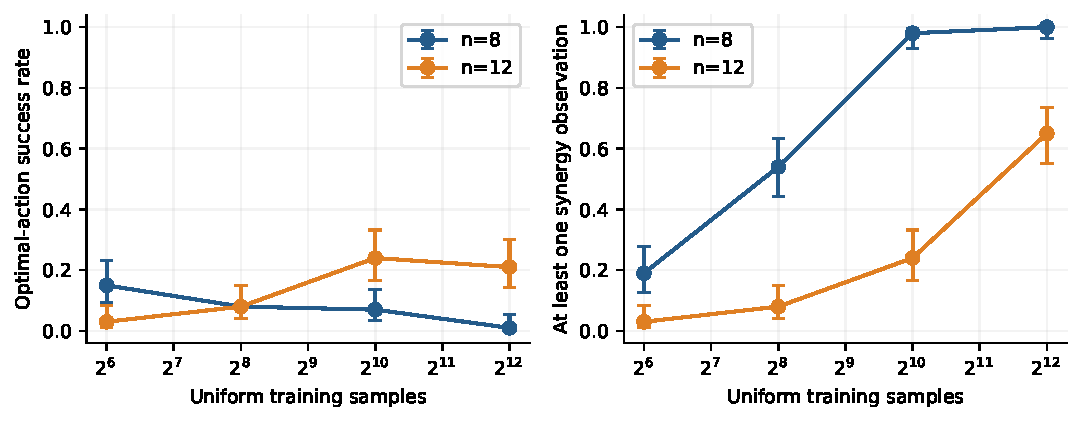
\includegraphics[width=0.86\linewidth]{../figures/sampling.pdf}
\caption{Uniform-sample additive fits: optimal-action success versus coverage of the synergy action, with Wilson 95\% intervals. Increased coverage need not repair the population projection's decision.}\label{fig:sampling}
\end{figure}

\subsection{Sanity checks}
Exactly representable additive and chain-pairwise control games reconstruct to numerical precision and choose optimal actions. An established $3\times3$ coordination game from QTRAN, also shown in Weighted QMIX, has reward matrix
\begin{equation}
 \begin{pmatrix}8&-12&-12\\-12&0&0\\-12&0&0\end{pmatrix}.
\end{equation}
Our additive row-plus-column least-squares projection chooses a zero-reward action, incurring regret eight. This checks the evaluator against a familiar pathology; it is not a reproduction of the QMIX or QTRAN algorithms. Independent weighted least-squares solves also verify (\ref{eq:anchor}), and complete-design least-squares solves verify the orthogonal projection and analytical MSE formulas.

\section{Discussion and limitations}
The strongest defensible conclusion is metric-specific: small absolute uniform reconstruction error alone is not a reliable decision certificate on the supplied games. Reporting normalization and decision regret makes this limitation visible. Pairwise factors improve the measured fit while preserving the wrong optimum because positive even-order interactions do not distinguish the all-zero and all-one configurations; unary coefficients break the symmetry in the wrong direction.

The construction is deliberately adversarial and highly symmetric. The interaction cost is scaled with agent count, and the rewarding joint event has exponentially small uniform probability. This choice produces a clean counterexample, not a realistic estimate of practical prevalence. The finite-sample study covers only two fixed games with deterministic rewards and uniform observations. Confidence intervals quantify dataset sampling only. We do not estimate across-task performance, noisy-reward robustness, partial observability, temporal credit assignment, dynamic graphs, or neural training behavior.

The oracle weighting ablation presupposes knowledge of the best joint action and cannot solve exploration. Its success therefore cannot be fairly compared with a learner receiving only sampled global rewards. Graph models are granted central exhaustive maximization, and action spaces beyond the reported range may be intractable. We evaluate no LOMAQ, VDN, QMIX, QTRAN, DCG, or recent neural baseline. The matrix game supplies a published diagnostic reference but does not replace validation in an established sequential environment.

This is a finished scoped diagnostic manuscript, not a submission-ready full MARL study. Prior work already establishes the central conceptual limitation. A stronger publication contribution would need a distinct unresolved result, a faithful implementation of relevant baselines, and independently reviewed evidence on sequential cooperative tasks. We make no acceptance, endorsement, or state-of-the-art claim.

\section{Conclusion}
A reproducible family separates uniform reward reconstruction from cooperative action quality: exact additive and pairwise projections can have vanishing absolute MSE and nearly unit regret. Normalized error exposes the missed reward variation; a privileged weighting ablation demonstrates the different preferences of prediction and decision objectives. The code, proofs, and retained experiments make this established concern directly inspectable and define a transparent starting point for broader validation.

\paragraph{AI assistance and authorship.}
AI tools assisted with literature lookup, study design, proofs, implementation, execution, and manuscript drafting. The displayed author name is supplied for the user's review; no affiliation, coauthor, supervisor involvement, or independent human validation is asserted. The author must review the work and decide authorship and disclosure before any external submission. No text, experimental metrics, or private artifacts from the author's prior project reports are reused as new evidence.

\bibliographystyle{plainnat}
\bibliography{references}

\appendix
\section{Reproduction and artifact map}
From the repository root, create a Python 3.12 environment, install \texttt{requirements-lock.txt}, and run:
\begin{verbatim}
python -m pytest -q
python -m src.run --config configs/full.json --output reproduction/full
python -m src.analyze --results reproduction/full \
  --figures reproduction/figures --tables reproduction/tables
\end{verbatim}
The runner refuses to overwrite a completed run. The original evidence is in \texttt{results/full/}: \texttt{exact.csv}, \texttt{sampling.csv}, \texttt{controls.csv}, the published matrix check, and a manifest. \texttt{results/pilot/} is separately retained. All manuscript tables and figures are generated by \texttt{src/analyze.py}; \texttt{docs/claim-evidence.md} maps quantitative statements to their rows. Deterministic content can be compared independently of timing fields. Numerical results may differ slightly across BLAS implementations, while the tested decisions and analytic identities should agree within floating-point tolerance.

\section{Greedy regret bound}
For completeness, let $a^*$ maximize $R$ and $\widehat a$ maximize $\widehat R$. Then
\begin{align*}
 R(a^*)-R(\widehat a)
 &=R(a^*)-\widehat R(a^*)+\widehat R(a^*)-\widehat R(\widehat a)
   +\widehat R(\widehat a)-R(\widehat a)\\
 &\leq |R(a^*)-\widehat R(a^*)|+|\widehat R(\widehat a)-R(\widehat a)|
 \leq2\|R-\widehat R\|_\infty.
\end{align*}
Since each action contributes its squared error divided by $2^n$ to uniform MSE, $\|R-\widehat R\|_\infty\leq\sqrt{2^nL}$. The exponential coverage factor explains why small average error alone does not certify the decisions in the counterexample.
\end{document}
